% !TEX root = *.root.tex

\documentclass[Análisis.root.tex]{subfiles}

\usetikzlibrary{positioning,shapes,fit,arrows}

\begin{document}
    \section{Números reales y Funciones}
    \subsection{Números reales}
        Hasta el momento conocemos distintos conjuntos de números:
        \begin{itemize}
            \item Naturales, $\mathbb{N} = \{1,2,3,4,...\}$
            \item Enteros, $\mathbb{Z} = \{...,-2,-1,0,1,2,...\}$
            \item Racionales, $\mathbb{Q} = \{\frac{a}{b} / a \in \mathbb{Z}; b \in \mathbb{Z};b \ne 0\}$
        \end{itemize}
        Cada uno de estos conjuntos resulta estar incluido en el anterior: $\mathbb{N} \subset \mathbb{Z} \subset \mathbb{Q} \subset \mathbb{R}$
        \begin{center}
            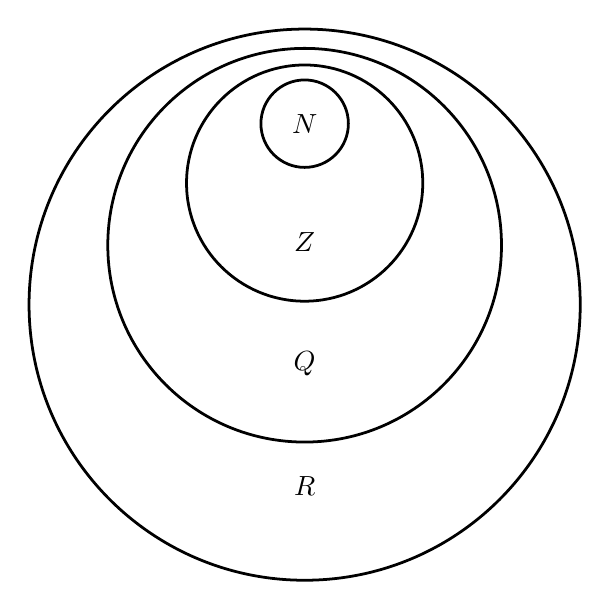
\begin{tikzpicture}[line width=1pt]
                \node (n) {$\mathbb{N}$};
                \node [below=of n] (z) {$\mathbb{Z}$};
                \node [below=of z] (q) {$\mathbb{Q}$};
                \node [below=of q] (r) {$\mathbb{R}$};

                \node[shape=circle,draw=black,fit={(n)}] {};
                \node[shape=circle,draw=black,minimum size=3cm,fit={(n) (z)}] {};
                \node[shape=circle,draw=black,minimum size=5cm,fit={(n) (q)}] {};
                \node[shape=circle,draw=black,minimum size=7cm,fit={(n) (r)}] {};

                \draw (n) (z) (q) (r);
            \end{tikzpicture}
        \end{center}
    \subsection{Funciones}
        Una función $f: A \rightarrow B$ es una relación entre dos conjuntos, donde cada elemento del conjunto $A$ señala un sólo elemento del conjunto $B$.
        \begin{center}
            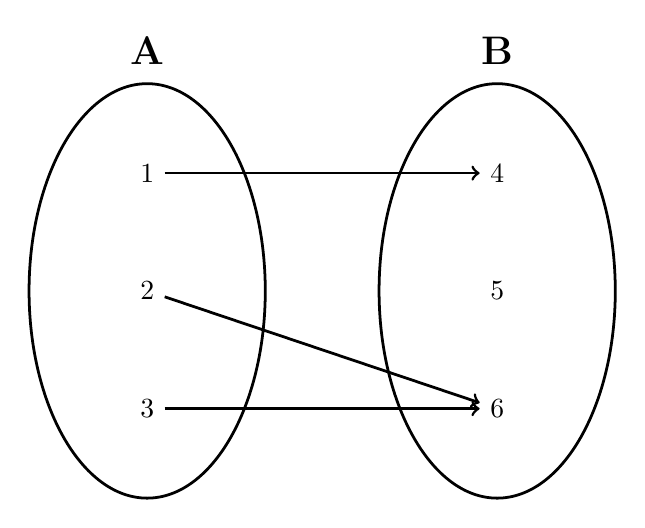
\begin{tikzpicture}[line width=1pt]
                \node (a1) {1};
                \node[below=of a1] (a2) {2};
                \node[below=of a2] (a3) {3};

                \node[right=4cm of a1] (b1) {4};
                \node[below=of b1] (b2) {5};
                \node[below=of b2] (b3) {6};

                \node[shape=ellipse,draw=black,minimum size=3cm,fit={(a1) (a3)}] {};
                \node[shape=ellipse,draw=black,minimum size=3cm,fit={(b1) (b3)}] {};

                \node[above=1cm of a1,font=\Large\bfseries] {A};
                \node[above=1cm of b1,font=\Large\bfseries] {B};

                \draw[->] (a1) -- (b1);
                \draw[->] (a2) -- (b3);
                \draw[->] (a3) -- (b3);
            \end{tikzpicture}
        \end{center}
        Se puede evaluar la función así:
        \begin{center}
            \begin{tabularx}{\textwidth}{XXX}
                \centering{$f(1) = 4$} & \centering{$f(2) = 6$} & \centering{$f(3) = 6$}\\
            \end{tabularx}
        \end{center}
        Como se puede ver, siempre hay un resultado por cada evaluación, no importa si hay dos o más elementos del conjunto $A$ cuya evaluación tenga el mismo resultado.\\
        En caso contrario, no sería una función, sería una relación no funcional, como el siguiente ejemplo:
        \begin{center}
            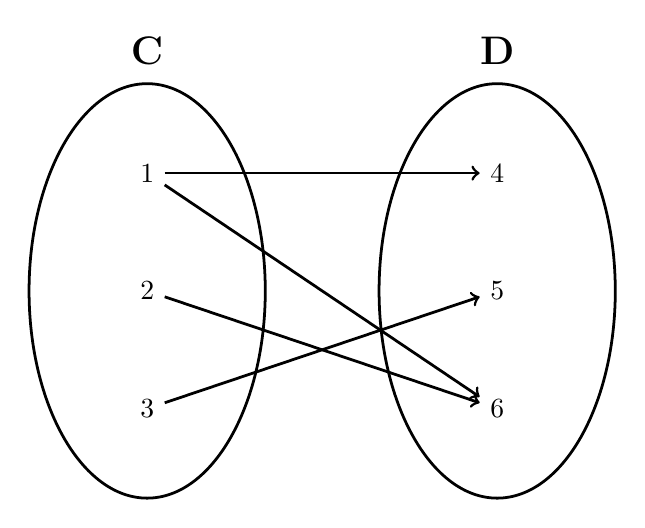
\begin{tikzpicture}[line width=1pt]
                \node (a1) {1};
                \node[below=of a1] (a2) {2};
                \node[below=of a2] (a3) {3};

                \node[right=4cm of a1] (b1) {4};
                \node[below=of b1] (b2) {5};
                \node[below=of b2] (b3) {6};

                \node[shape=ellipse,draw=black,minimum size=3cm,fit={(a1) (a3)}] {};
                \node[shape=ellipse,draw=black,minimum size=3cm,fit={(b1) (b3)}] {};

                \node[above=1cm of a1,font=\Large\bfseries] {C};
                \node[above=1cm of b1,font=\Large\bfseries] {D};

                \draw[->] (a1) -- (b1);
                \draw[->] (a2) -- (b3);
                \draw[->] (a1) -- (b3);
                \draw[->] (a3) -- (b2);
            \end{tikzpicture}
        \end{center}
        Volviendo a las funciones, a todo conjunto de salida se lo denomina el Dominio de una función, en este caso:
        \begin{center}
            $Dom f = A$
        \end{center}
        Por su parte, al conjunto de llegada se lo llama el Codominio de una función:
        \begin{center}
            $Codom f = B$
        \end{center}
\end{document}